\documentclass[11pt]{article}
\usepackage[T1]{fontenc}
\usepackage{lmodern}
\usepackage[margin=1in]{geometry}
\usepackage{amsmath,amssymb,bm,booktabs,tabularx,array}
\IfFileExists{microtype.sty}{\usepackage{microtype}}{}
\usepackage[dvipsnames]{xcolor}
\usepackage{tikz}
\usetikzlibrary{arrows.meta,positioning}
\usepackage{hyperref}
\definecolor{ink}{HTML}{193549}
\definecolor{accent}{HTML}{007C83}
\hypersetup{colorlinks=true,linkcolor=ink,urlcolor=accent,citecolor=accent,
 pdftitle={From JIRAM images to winds: a pedagogical companion to Ingersoll et al. (2022)}}
\setlength{\parindent}{0pt}
\setlength{\parskip}{0.55em}
\setlength{\emergencystretch}{2em}
\newcommand{\vel}{\bm{v}}
\newcommand{\pos}{\bm{x}}
\newcommand{\disp}{\bm{d}}
\newcommand{\Var}{\operatorname{Var}}
\newcommand{\Cov}{\operatorname{Cov}}
\newcommand{\rms}{\operatorname{rms}}
\newcommand{\ms}{\mathrm{m\,s^{-1}}}
\newcommand{\sone}{\mathrm{s^{-1}}}
\newenvironment{teaching}[1]{\begin{quote}\small\textbf{#1}\par}{\end{quote}}
\title{\color{ink}From JIRAM images to winds\\[0.35em]
 \large A pedagogical companion to Ingersoll et al. (2022)}
\author{Methods notes for the \texttt{jiram\_catalog} project}
\date{9 September 2026}

\begin{document}
\maketitle
\begin{abstract}
Cloud tracking estimates the displacement of a brightness pattern. Turning
that estimate into an atmospheric measurement requires a coordinate system,
a time interval, a definition of the scale being measured, and an error model.
This note develops those connections from elementary examples, motivated by
the north-polar JIRAM analysis of Ingersoll and colleagues. It then identifies
which building blocks our repository already has and which proposed features
would make the resulting science easier to assess.
\end{abstract}

\textbf{How to read this note.} Section~\ref{sec:recipe} is a compact record
of the publication's reported recipe. The mathematical development that
follows is an original teaching reconstruction, not the authors' software
documentation. Worked examples are synthetic. Repository observations and
future proposals are explicitly labelled. No new velocity retrieval has been
run for this document.

\tableofcontents
\newpage

\section{The measurement we are trying to make}

Imagine two photographs of patterned fabric on a moving conveyor belt.
Recognizing the same patch in both photographs gives a displacement. A ruler
converts pixels into metres; a clock converts displacement into velocity.
Cloud tracking has the same structure, with complications: the camera moves,
the surface is curved, the texture changes, and the material can deform.

An image is a scalar field $I(\pos,t)$. A horizontal velocity has two
components, $\vel=(u,v)$. The central inference is
\begin{equation}
 I(\pos,t)\ \longrightarrow\ \widehat{\disp}(\pos;t_0,t_1)
 \ \longrightarrow\ \widehat{\vel}(\pos)
 \ \longrightarrow\ \widehat{\zeta},\widehat{D},
\end{equation}
where hats indicate estimates, $\zeta$ denotes relative vorticity, and $D$
denotes horizontal divergence. Each arrow adds a requirement. In particular,
the last arrow differentiates velocity and magnifies spatially varying errors.

Brightness patterns are tracers, not tagged air parcels. Even perfectly
measured pattern motion can differ from material motion when clouds form,
evaporate, change optical properties, or contain propagating waves. A useful
workflow therefore keeps \emph{image displacement}, \emph{inferred wind}, and
\emph{dynamical interpretation} as distinct products.

\section{The published recipe, in one place}\label{sec:recipe}

The paper is \emph{Vorticity and divergence at scales down to 200 km within
and around the polar cyclones of Jupiter}, in \emph{Nature Astronomy}, not
\emph{Nature Astrophysics}~\cite{ingersoll}.

\begin{center}
\small
\begin{tabularx}{\linewidth}{@{}p{0.27\linewidth}X@{}}
\toprule
Element & Reported choice \\
\midrule
Observations & JIRAM M-band, 2 February 2017; four sets of twelve images. \\
Mapping & SPICE/instrument geometry; polar orthographic plane; 15 km pixels. \\
Pairing & n01--n03 and n02--n04; approximately 16 minutes per pair,
with actual image times; estimates approximately 8 minutes apart. \\
Tracker & JPL Tracker3; brightness correlation in $15\times15$ pixel
patches (225 km sides). \\
Velocity sampling & 45 km; native image sampling changes from 22 to 14 km. \\
Quality & Mask low-entropy patches; 256 brightness bins per patch. \\
Derivatives & Circulation and outward-flux integrals; square sides
90, 180, 270, 360 km. \\
Noise assessment & Compare disjoint image-pair estimates; fitted
velocity-component uncertainty about $7.8\,\ms$. \\
\bottomrule
\end{tabularx}
\end{center}

At the 180 km diagnostic scale, repeat-estimate correlations were about
0.729 for vorticity and 0.299 for divergence. The analysis supported
anticyclonic shielding but did not detect the proposed divergence--anticyclonic
vorticity correlation at its resolved scales. See Methods, Figs.~2--3, and
Table~1 of the article~\cite{ingersoll}.

\section{First establish what a pixel means}

\subsection{Geometry precedes tracking}

For a detector pixel, a geometric mapper uses the instrument model,
spacecraft attitude and position, time, and a reference planetary surface to
construct a viewing ray and its surface intersection. A projection then
places that intersection on a common map. This removes predicted camera
motion before cloud motion is estimated. Reprojection must preserve missing
coverage as a mask; filling a gap with black creates an artificial feature.

Let a map have coordinates $(x,y)$ in metres. For a locally Cartesian grid,
with pixel spacings $s_x,s_y$, a measured displacement $(d_x,d_y)$ in pixels
becomes
\begin{equation}\label{eq:velocity}
 \widehat{u}=\frac{s_xd_x}{\Delta t},\qquad
 \widehat{v}=\frac{s_yd_y}{\Delta t},\qquad \Delta t=t_1-t_0.
\end{equation}
An array row is not automatically geographic north. Its direction can even
oppose the map's positive vertical axis. A polar map also rotates the local
east/north basis as longitude changes.

For an arbitrary projection, write the local relationship as
\begin{equation}
 \begin{pmatrix}\dot x\\\dot y\end{pmatrix}
 =\mathsf{J}(\lambda,\phi)
 \begin{pmatrix}u_E\\v_N\end{pmatrix},
\end{equation}
where $\mathsf{J}$ is the projection Jacobian with respect to physical east
and north distances. Invert this relationship to report east/north winds
where the map is nonsingular. A simple map-plane derivative is a local
approximation to a surface derivative. On a wide polar domain the metric
must be included, or its neglected error quantified. An orthographic map
preserves neither all distances nor all areas.

\subsection{A mosaic is not necessarily an instant}

A tiled image can contain observations acquired at different times. Preserve
the source identity and acquisition time behind each tracked patch. When
two patches use different source images, their $\Delta t$ can differ even if
both belong to the same nominal pair of mosaics. A cumulative display
mosaic can also repeat old pixels; repeated display frames do not constitute
independent exposures.

\begin{teaching}{Worked example: units and navigation bias}
Choose a synthetic grid with $s_x=s_y=20{,}000$ m and $\Delta t=900$ s.
A displacement $(2.4,-1.2)$ pixels gives
$(u,v)=(53.33,-26.67)\,\ms$. A relative navigation offset of just 0.5 pixel
adds $11.11\,\ms$ along the affected axis. Correlation cannot distinguish
that offset from a uniform translation of the clouds without independent
geometric information.
\end{teaching}

\section{How a correlation tracker measures a displacement}

\subsection{Turn a patch into a search problem}

Choose a template patch $A_i$ in the first image. For each trial displacement
$\disp$, compare it with a patch $B_i(\disp)$ in the second. A standard,
useful realization is normalized cross-correlation:
\begin{equation}\label{eq:ncc}
 C(\disp)=
 \frac{\sum_{i\in M(\disp)}(A_i-\bar A)(B_i(\disp)-\bar B)}
 {\left[\sum_{i\in M(\disp)}(A_i-\bar A)^2
 \sum_{i\in M(\disp)}(B_i(\disp)-\bar B)^2\right]^{1/2}}.
\end{equation}
The means use the same jointly valid set $M(\disp)$ as the sums. The mask
changes with displacement. Require adequate support and nonzero variance;
otherwise the score can be undefined or based on too few samples.

The selected displacement maximizes $C$. Subtracting the mean makes the
score insensitive to a constant brightness offset; dividing by the standard
deviations removes a positive multiplicative gain. Neither operation corrects
changing shadows, local radiometric distortion, or genuine cloud evolution.

An integer search can be refined near its maximum. For example, fit
$q(\bm{\epsilon})=a+\bm{b}^{T}\bm{\epsilon}
+\tfrac12\bm{\epsilon}^{T}\mathsf{H}\bm{\epsilon}$ to nearby correlation
scores. If $\mathsf{H}$ is negative definite and the fitted maximum is nearby,
then $\bm{\epsilon}_*=-\mathsf{H}^{-1}\bm{b}$ provides a subpixel correction.
This is interpolation of a measured peak, not evidence for arbitrarily fine
spatial resolution.

Equation~\eqref{eq:ncc} and this refinement describe the local
reimplementation inspected for this note~\cite{repotracker}. They are a
concrete teaching model; the publication does not establish that every
normalization, peak-fitting, or rejection choice is identical in its tracker.

\subsection{Why this belongs to the optical-flow family}

The simplest brightness-advection model is
\begin{equation}\label{eq:advect}
 I(\pos+\vel\Delta t,t+\Delta t)\simeq I(\pos,t).
\end{equation}
A first-order expansion gives
\begin{equation}\label{eq:of}
 I_t+uI_x+vI_y\simeq0.
\end{equation}
There is only one scalar equation for two unknown components at a pixel.
This is the aperture problem: a straight stripe moving along itself is
locally indistinguishable from a stationary stripe. A textured patch
provides gradients in several directions, making a common local displacement
estimable.

Patch correlation searches finite displacements. A differential optical-flow
method solves a version of Eq.~\eqref{eq:of}, often with neighborhood or
smoothness assumptions. A learned model obtains additional constraints from
training data and its architecture. These are different ways to resolve
ambiguity; a dense output array alone does not show which displacements were
well constrained by the images.

More generally the image can obey
\begin{equation}
 I_t+\vel\cdot\nabla I=S_I,
\end{equation}
with a source term $S_I$ representing changing tracer brightness. Setting
$S_I=0$ is an assumption. A model may fit the images very well while assigning
some of $S_I$ to a spurious velocity.

\section{Texture determines where a vector is credible}

Shannon entropy of a patch histogram is
\begin{equation}
 H=-\sum_{k:p_k>0}p_k\log_2p_k.
\end{equation}
If all samples occupy one bin, $H=0$. If $N$ samples occupy distinct bins,
$H=\log_2N$, provided at least $N$ bins are available. This counts occupied
intensity states, not spatial arrangements.

Consequently a monotonic ramp can have a broad histogram while constraining
motion in only one direction. Random detector noise can have high entropy
without persistent texture. Histogram entropy is useful as one diagnostic,
but it is not a probability that a vector is correct. Its numerical threshold
depends on binning, intensity scaling, and patch size.

A complementary mathematical diagnostic is the structure tensor
\begin{equation}
 \mathsf{G}=\sum_i w_i
 \begin{pmatrix}I_{x,i}^2&I_{x,i}I_{y,i}\\
 I_{x,i}I_{y,i}&I_{y,i}^2\end{pmatrix}.
\end{equation}
Two appreciable eigenvalues imply sensitivity to both displacement
components. One very small eigenvalue indicates an aperture ambiguity.
This is a suggested additional check, not a reported ingredient of the
publication's workflow.

Other useful proposed diagnostics are a distinct correlation peak, distance
from the search boundary, common valid area, and forward/backward agreement.
For the last check, let $\bm{p}$ and both displacements be in pixel units,
and evaluate
\begin{equation}
 \bm{r}_{\rm FB}(\bm{p})=\disp_{01}(\bm{p})
 +\disp_{10}\bigl(\bm{p}+\disp_{01}(\bm{p})\bigr).
\end{equation}
Consistent correspondence gives a small residual. It still cannot rule out
a systematic error common to both directions.

\section{Four spatial scales that should never share one label}

\begin{enumerate}
 \item \textbf{Native image sampling:} the physical distance between
 detector samples on the planet. It changes with viewing geometry.
 \item \textbf{Map pixel spacing:} the interval of the resampled coordinate
 grid. Making this smaller creates additional interpolated samples.
 \item \textbf{Template support and vector spacing:} a velocity uses texture
 throughout its patch; neighboring vector locations may use heavily
 overlapping patches. Support and spacing are separate quantities.
 \item \textbf{Derivative scale:} the area or stencil over which velocity
 variations are converted into vorticity or divergence.
\end{enumerate}

The values for the experiment are collected in Section~\ref{sec:recipe}.
Its template width is five output-grid intervals. That ratio immediately
warns against treating neighboring vectors as independent measurements.
A half-width convention for wind localization should not be mistaken for
a measured Fourier transfer function.

\begin{teaching}{An oversampling thought experiment}
Take a synthetic image whose useful texture exists only in 240 km patches.
Evaluate a translation estimate every 40 km, then repeat every 10 km.
The second display has sixteen times as many arrows per unit area.
It has acquired no new photons and need not resolve any smaller eddies.
It can still be useful for rendering and numerical integration, provided
its dependence between neighboring estimates is retained.
\end{teaching}

One approximate mental model is
\begin{equation}
 \widehat{\vel}\simeq K*\vel+\bm{e},
\end{equation}
where $K$ represents spatial averaging and $\bm{e}$ error. A correlation
estimator is nonlinear, so $K$ is generally texture- and flow-dependent;
it is not automatically a square top-hat the size of the template. Synthetic
advection with known velocity is a way to measure the effective response.

\section{From velocity to vorticity and divergence}

\subsection{Physical definitions}

On a Cartesian tangent plane with $x$ rightwards, $y$ upwards, and positive
normal out of the page,
\begin{equation}\label{eq:derivatives}
 \zeta=\frac{\partial v}{\partial x}-\frac{\partial u}{\partial y},
 \qquad
 D=\frac{\partial u}{\partial x}+\frac{\partial v}{\partial y}.
\end{equation}
Positive $\zeta$ is counterclockwise rotation. Positive $D$ means horizontal
outflow from a small region. Both have units $\sone$.

\subsection{Measure a finite-area quantity using its boundary}

For a region $A$ with counterclockwise boundary $\partial A$, Stokes's and
the planar divergence theorems give
\begin{align}
 \bar\zeta_A&=\frac{1}{|A|}\oint_{\partial A}(u\,dx+v\,dy),
 \label{eq:curlcontour}\\
 \bar D_A&=\frac{1}{|A|}\oint_{\partial A}(u\,dy-v\,dx).
 \label{eq:divcontour}
\end{align}
The first integral measures circulation along the boundary. The second
measures flow across it, positive outwards. Division by area converts these
integrated quantities into area-mean derivatives. These equations do not
recover a point value at unlimited resolution.

\begin{center}
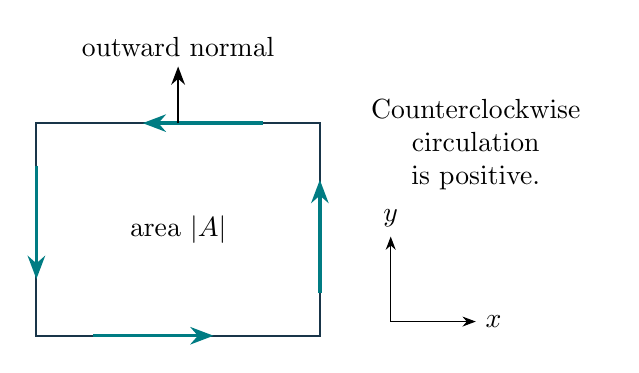
\begin{tikzpicture}[scale=0.9,>=Stealth]
 \draw[thick,ink] (0,0) rectangle (4,3);
 \draw[->,very thick,accent] (0.8,0) -- (2.5,0);
 \draw[->,very thick,accent] (4,0.6) -- (4,2.2);
 \draw[->,very thick,accent] (3.2,3) -- (1.5,3);
 \draw[->,very thick,accent] (0,2.4) -- (0,0.8);
 \draw[->,thick] (2,3) -- (2,3.8) node[above] {outward normal};
 \node at (2,1.5) {area $|A|$};
 \draw[->] (5,0.2) -- (6.2,0.2) node[right] {$x$};
 \draw[->] (5,0.2) -- (5,1.4) node[above] {$y$};
 \node[align=center,text width=3.2cm] at (6.2,2.7)
 {Counterclockwise\\circulation is positive.};
\end{tikzpicture}
\end{center}

For a square of side $L$, a transparent approximation using edge-mean
velocities is
\begin{align}
 \bar\zeta&\simeq
 \frac{\bar v_R-\bar v_L-\bar u_T+\bar u_B}{L},\\
 \bar D&\simeq
 \frac{\bar u_R-\bar u_L+\bar v_T-\bar v_B}{L}.
\end{align}
Here $R,L,T,B$ denote right, left, top, and bottom edges; the symbol $L$
in the denominator denotes length. These are teaching approximations, not
a claim about the authors' exact quadrature or interpolation rules.

An implementation should evaluate velocities along the complete supported
contour. Replacing a missing edge by zero invents a circulation or flux.
Interpolation across a small gap needs an explicit rule and uncertainty;
unsupported contours should otherwise remain masked.

\subsection{Three fields that expose sign and scale errors}

\begin{center}
\begin{tabular}{@{}llll@{}}
\toprule
Field & Velocity & Vorticity & Divergence \\
\midrule
Translation & $(U,V)$ & $0$ & $0$ \\
Rigid rotation & $(-\omega y,\omega x)$ & $2\omega$ & $0$ \\
Isotropic expansion & $(\alpha x,\alpha y)$ & $0$ & $2\alpha$ \\
\bottomrule
\end{tabular}
\end{center}

These exact identities provide independent checks for either finite
differences or contour integration. They also show why a spatially uniform
navigation shift biases velocity but leaves ideal derivatives unchanged,
whereas a rotation, scale change, or discontinuous tile offset can create
false vorticity or divergence.

\section{Why derivative uncertainty needs its own analysis}

If each image's position estimate has independent component uncertainty
$\sigma_x$ in metres, then differencing two positions gives
\begin{equation}
 \sigma_u=\frac{\sqrt{2}\,\sigma_x}{\Delta t}.
\end{equation}
Longer baselines reduce this localization contribution while increasing the
opportunity for deformation and tracer evolution. There is therefore an
observational optimum, not a rule that the longest baseline is best.

If the four relevant edge-mean components in the square approximation have
independent, equal uncertainty $\sigma_e$, then
\begin{equation}\label{eq:toyerror}
 \sigma_{\bar D}=\sigma_{\bar\zeta}=\frac{2\sigma_e}{L}.
\end{equation}
This illustrative formula applies to \emph{edge means}; substituting a
single-vector uncertainty silently assumes those edge means have that same
uncertainty. Overlapping templates and reused contour samples normally
introduce covariance.

For any linear discretized diagnostic $q=\bm{w}^{T}\bm{z}$, the general
propagation rule is
\begin{equation}
 \Var(q)=\bm{w}^{T}\mathsf{C}\bm{w},
\end{equation}
where $\mathsf{C}$ is the covariance of the velocity samples. Oversampling
does not justify setting the off-diagonal entries to zero.

\begin{teaching}{Worked example: a plausible wind error can dominate divergence}
On the synthetic grid used earlier, 0.2-pixel position uncertainty in each
image gives $\sigma_u=6.29\,\ms$. If, purely for illustration, each of four
independent edge means has this uncertainty, a 200 km square gives
$\sigma_{\bar D}=6.29\times10^{-5}\,\sone$. A true divergence of
$2\times10^{-5}\,\sone$ is then smaller than the noise in one estimate,
even though a $60\,\ms$ wind may look convincing. The edge-independence
assumption is part of this example, not a calibration for Jupiter.
\end{teaching}

\section{Use repeated measurements to separate signal and noise}

\subsection{Why four image sets are valuable}

Consider equally spaced synthetic observations at $t_0,t_0+\tau,
t_0+2\tau,t_0+3\tau$. Form velocities from images $1\to3$ and $2\to4$:

\begin{center}
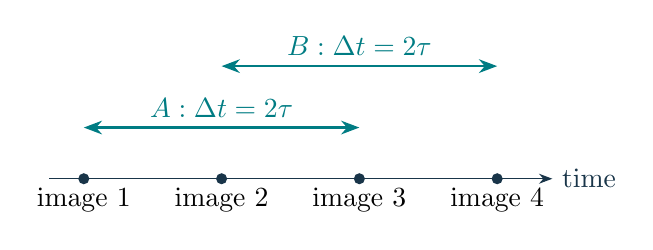
\begin{tikzpicture}[>=Stealth,x=1.75cm,y=0.65cm]
 \draw[->,ink] (-0.25,0) -- (3.4,0) node[right] {time};
 \foreach \x/\n in {0/1,1/2,2/3,3/4}{
   \fill[ink] (\x,0) circle (2pt);
   \node[below] at (\x,0) {image \n};}
 \draw[<->,thick,accent] (0,1) -- (2,1)
   node[midway,above] {$A: \Delta t=2\tau$};
 \draw[<->,thick,accent] (1,2.2) -- (3,2.2)
   node[midway,above] {$B: \Delta t=2\tau$};
\end{tikzpicture}
\end{center}

The two estimates have equal baselines, midpoints separated by $\tau$, and
no input image in common. If structures change little over $\tau$, the
estimates can be treated approximately as repeat measurements of one field.
This is a physical assumption to assess at the chosen diagnostic scale.

\subsection{Derive the covariance estimator}

Let $A=s+e_A$ and $B=s+e_B$ be two mean-subtracted estimates of a diagnostic.
Assume errors are uncorrelated with $s$, uncorrelated with each other, and
have equal variance $\sigma_n^2$. Then
\begin{align}
 \Var(A)=\Var(B)&=\sigma_s^2+\sigma_n^2,\\
 \Cov(A,B)&=\sigma_s^2,\\
 \eta=\operatorname{corr}(A,B)&=
 \frac{\sigma_s^2}{\sigma_s^2+\sigma_n^2}.
\end{align}
Thus $\eta$ is the signal fraction of \emph{variance} under this model,
not a fraction of pixels that are correct and not a fraction of amplitude.

Another original way to see the same algebra is to form
$S=(A+B)/2$ and $N=(A-B)/2$. Under those assumptions,
\begin{equation}
 \Var(N)=\frac{\sigma_n^2}{2},\qquad
 \Var(S)=\sigma_s^2+\frac{\sigma_n^2}{2},\qquad
 \sigma_s^2=\Var(S)-\Var(N).
\end{equation}
The difference estimates the noise of the \emph{averaged} measurement.
For unequal individual noise levels, $\Var(A)-\Cov(A,B)$ and
$\Var(B)-\Cov(A,B)$ estimate their separate noise variances if the other
assumptions still hold. Negative estimates in finite samples flag instability
or model mismatch; they should not silently become evidence of no noise.

\begin{teaching}{Worked example: interpret a correlation correctly}
Suppose each measurement has standard deviation $10$ in arbitrary diagnostic
units and their correlation is 0.36. Their covariance is 36, so the common
signal standard deviation is $6$ and the individual noise standard deviation
is $8$. Averaging the pair reduces the independent noise standard deviation
to $8/\sqrt2=5.66$; the signal remains $6$. These figures are synthetic.
\end{teaching}

\subsection{What disjoint inputs do not guarantee}

For evolving signals $s_A,s_B$, the covariance instead contains
\begin{equation}
 \Cov(A,B)=\Cov(s_A,s_B)+\Cov(e_A,e_B)
 +\Cov(s_A,e_B)+\Cov(e_A,s_B).
\end{equation}
Common navigation or calibration errors can survive in the covariance and
masquerade as a repeatable signal. Real evolution can reduce signal
covariance, making a discrepancy look like measurement noise. Correlation
failures that depend systematically on the same texture can also recur.

Shared images cause an additional, explicit dependence. If image position
errors $p_1,p_2,p_3$ are independent with variance $\sigma_p^2$, adjacent
velocity errors are
\begin{equation}
 e_{12}=\frac{p_2-p_1}{\Delta t},\qquad
 e_{23}=\frac{p_3-p_2}{\Delta t},\qquad
 \Cov(e_{12},e_{23})=-\frac{\sigma_p^2}{\Delta t^2}.
\end{equation}
Pairs sharing an image are consequently not interchangeable with disjoint
pairs in a noise calculation. Even the disjoint-pair calculation needs common
spatial support, comparable temporal averaging, and uncertainty estimates
that respect dependence among neighboring vectors.

\section{What physical conclusions require beyond image tracking}

\subsection{Shielding is a velocity-gradient statement}

For an ideal axisymmetric vortex with azimuthal wind $v_\theta(r)$,
\begin{equation}
 \zeta(r)=\frac{1}{r}\frac{d(rv_\theta)}{dr}.
\end{equation}
An annulus can therefore have negative vorticity even while
$v_\theta>0$: the velocity merely has to decrease faster than $1/r$.
For the synthetic profile $v_\theta=Cr^{-p}$,
$\zeta=(1-p)Cr^{-p-1}$, which is negative for $C>0$ and $p>1$.
This explains how to interpret an anticyclonic shielding ring without
requiring every wind arrow in that ring to reverse direction.

\subsection{Divergence is not a direct vertical-velocity measurement}

For a simple incompressible three-dimensional flow,
\begin{equation}
 D=-\frac{\partial w}{\partial z}.
\end{equation}
This constrains a vertical gradient, not $w$ at a cloud level. A compressible
atmosphere requires density-weighted continuity and information about vertical
structure. Likewise, failure to detect a zero-lag correlation does not prove
that a physical mechanism is absent: two causally related oscillatory
signals can have zero correlation if one is a quarter cycle out of phase.

Siegelman et al. (2022) also analyzed these polar observations, combining
tracked winds with infrared optical-depth anomalies and a surface
quasigeostrophic interpretation to investigate smaller-scale convection and
energy transfer~\cite{siegelman}. Treat this as a distinct inference chain:
the brightness field becomes a dynamical proxy under additional assumptions.
Changing those assumptions can change the inferred divergence even when the
input imagery is unchanged.

For this project, a direct velocity diagnostic and a model-assisted dynamical
reconstruction should carry distinct names, assumptions, and uncertainty
descriptions. Neither an attractive map nor a dense sampling grid establishes
that a small-scale energy-transfer estimate is resolved.

\section{Where our repository already stands}\label{sec:repo}

The following statements are observations from the local code, saved
validation reports, and selected published-product headers; they are not
additional results of the journal article.

\subsection{A usable baseline exists, with measurable limitations}

\texttt{src/jiram\_catalog/tracking.py} implements masked normalized
cross-correlation, subpixel peak refinement, and a reader for the published
vector tables. Defaults include a 15-pixel square template, 35 trial-centre
offsets per axis, at least 90\% common valid support, and NCC at least 0.5.
The 35 offsets span $-17$ to $+17$ pixels; this is our implementation's
search convention. A peak at the search edge is retained without subpixel
refinement. These choices do not establish identity with the original
software~\cite{repotracker}.

The existing PJ4 report compares 24 corresponding same-letter tile pairs
at subsampled published vector positions:
\begin{center}
\small
\begin{tabularx}{\linewidth}{@{}Xrrr@{}}
\toprule
Input to our tracker & Median error & 90th percentile & Within 1 pixel \\
\midrule
Published maps & 0.224 px & 4.759 px & 83.4\% \\
Our reprojections & 0.434 px & 4.685 px & 80.1\% \\
\bottomrule
\end{tabularx}
\end{center}
The corresponding median vector-difference magnitudes are 3.45 and
$6.69\,\ms$. These are $\|\vel_{\rm ours}-\vel_{\rm reference}\|$, not
differences between scalar speeds~\cite{repovalidation}. The medians provide
encouraging agreement; the tails make clear that a single typical error
cannot describe the whole field. The reference vectors are a published
comparison standard, not an independent measurement of exact atmospheric
truth. These saved results were inspected, not regenerated for this note.

The existing tracking gate checks saved summary metrics. It does not rerun
all tracking or establish vorticity/divergence accuracy. The current GUI
registration action estimates a bounded image displacement; its vector route
loads an already associated vector product. Neither is a complete dense-wind
retrieval and derivative-analysis workflow~\cite{repoapi}.

\subsection{Three provenance details worth resolving before reproduction}

\begin{enumerate}
 \item \textbf{Tracker name.} The paper names Tracker3. The inspected
 \texttt{n0103aa.tp4} history contains \texttt{TASK='TRACKER4'}.
 Preserve both facts; source/version equivalence is unresolved.
 \item \textbf{Vector sampling.} That raw table records \texttt{GRID=1},
 \texttt{MPS=15}, and dense integer template positions. The published
 analysis spacing and the raw table's placement spacing are therefore
 different stages. The precise selection or aggregation producing the
 analysis grid needs verification. The folder name's ``45 km'' must not
 be interpreted as cloud altitude; an early repository inventory made
 that unsupported inference.
 \item \textbf{Coordinates and clocks.} The example records
 \texttt{DT=974.002} s and sample/line displacement components. The
 repository reverses the line axis to match stored map rows. That reversal
 is empirically supported; the adopted one-based pixel origin is less
 strongly distinguished from a neighboring convention by tracking errors.
 Do not relabel these components as east/north without transformation.
 The repository's projection and region-array conventions also need a
 tested basis conversion: physical projection $y$ points opposite to image
 line, whereas generic region $y$ increases with row. A reflection can
 reverse the vorticity sign.
\end{enumerate}

The published maps and vectors are under the read-only \texttt{JIRAM}
reference directory configured by \texttt{JIRAM\_PAPER\_DATA}. They are
separate from the working \texttt{jiram\_mirror}. No files in either dataset
were changed for this note.

\section{Features I would build from these lessons}\label{sec:features}

These are proposals for later specification and implementation. Their order
reflects scientific dependencies.

\begin{enumerate}
 \item \textbf{A four-set experiment builder.} Select disjoint pairs with
 comparable baselines and common coverage. Show every source timestamp,
 the effective temporal support, band, map basis, and instrument eligibility.
 Reject repeated cumulative pixels as independent exposures.

 \item \textbf{A patch inspector.} Clicking an arrow should reveal the two
 patches, valid masks, correlation surface, subpixel fit, entropy, search
 boundary, and forward/backward residual. This makes a suspicious vector
 investigable instead of simply colouring it by a single score.

 \item \textbf{An associated velocity product.} Save source IDs and versions,
 pair times, displacement, physical components, projection basis, masks,
 diagnostics, method parameters, and uncertainty provenance. Connect that
 product explicitly to the time-series viewer and existing vector overlay.

 \item \textbf{Scale-aware derivative maps.} Offer circulation and flux
 diagnostics with the contour scale visible in kilometres. Display template
 support and vector spacing alongside it. Preserve unsupported contours and
 show noise estimates at each scale.

 \item \textbf{A repeatability panel.} Compare disjoint-pair fields using
 scatterplots, covariance, average/difference maps, and sensitivity to scale
 and masking. Label the stationary-signal and error-independence assumptions.
 Use spatial blocks or independent realizations when estimating confidence
 intervals, rather than counting every overlapping vector as independent.

 \item \textbf{A reproducible reference benchmark.} Begin with the published
 maps, then substitute our reprojections to isolate geometry contributions.
 Add synthetic translation, rotation, expansion, shear, missing coverage,
 brightness changes, and tile-offset cases. Compare the classical tracker
 with a proposed optical-flow model under matched sampling and filtering.
 Assess derivatives and effective resolution, not just displacement error.
\end{enumerate}

JIRAM M-band thermal-emission/cloud-opacity texture and reflected-light
JunoCam texture need different brightness-constancy checks.
For JunoCam, keep the existing instrument-failure exclusions and native-band
provenance. Timing, framelet assembly, limb/navigation residuals, and
illumination changes need instrument-specific checks before transporting
the JIRAM benchmark's confidence claims. A successfully exported tensor
does not establish accurate winds. The most useful first milestone is a
transparent PJ4 benchmark with associated vector products and scale-dependent
uncertainty; generalizing to other passes then has an explicit standard.

\section{Sources, access limits, and how to reproduce this note}

The full main article, including Methods, was read from the coauthor-hosted
PDF linked below. The publisher's supplementary-methods PDF could not be
retrieved in this session. The numerical entropy cutoff, detailed contour
quadrature, and any undocumented original Tracker settings are consequently
not asserted here. Selected local supplementary-data headers and the
repository's existing validation records provide the implementation evidence
described in Section~\ref{sec:repo}.

The document contains original schematics, derivations, and synthetic
examples; it reproduces no article figures. With a standard TeX installation,
compile from the repository root using:
\begin{quote}\small\ttfamily
pdflatex -output-directory=\$TMPDIR \\
\hspace*{1em}docs/pedagogy/ingersoll\_2022\_tracking.tex
\end{quote}
Run twice to resolve the table of contents and references. On Expanse,
\texttt{TMPDIR} must point to the configured Lustre scratch runtime directory.

\begin{thebibliography}{9}
\raggedright
\bibitem{ingersoll}
A. P. Ingersoll et al. (2022).
\emph{Vorticity and divergence at scales down to 200 km within and around
the polar cyclones of Jupiter}. Nature Astronomy \textbf{6}, 1280--1286.
\href{https://doi.org/10.1038/s41550-022-01774-0}{DOI: 10.1038/s41550-022-01774-0}.
\href{https://pordlabs.ucsd.edu/wryoung/reprintPDFs/VortDiv.pdf}{Coauthor-hosted full text}.
Specific locators: Methods, pp.~1284--1285; Fig.~2 caption; Table~1 and
Fig.~3; discussion of signal and noise, pp.~1281--1283.

\bibitem{siegelman}
L. Siegelman et al. (2022).
\emph{Moist convection drives an upscale energy transfer at Jovian high latitudes}.
Nature Physics \textbf{18}, 357--361.
\href{https://doi.org/10.1038/s41567-021-01458-y}{DOI: 10.1038/s41567-021-01458-y}.
See the discussion of optical-depth anomalies and the surface
quasigeostrophic framework.

\bibitem{repotracker}
Local repository: \texttt{src/jiram\_catalog/tracking.py}.
Inspected functions: \texttt{track\_pair}, \texttt{parabolic\_peak},
\texttt{read\_tp4}, and \texttt{match\_vectors}.
\href{https://github.com/ksr-ocean/jiram_catalog/blob/a6e3938e5c816583c49833791f7500e562acf155/src/jiram_catalog/tracking.py}{Versioned source}.

\bibitem{repovalidation}
Local repository: \texttt{docs/reports/tracking\_pj4.md};
\texttt{scripts/classical\_tracking\_pj4.py};
\texttt{tests/test\_gate\_tracking\_pj4.py}.
\href{https://github.com/ksr-ocean/jiram_catalog/blob/a6e3938e5c816583c49833791f7500e562acf155/docs/reports/tracking_pj4.md}{Versioned validation report}.
The historical \texttt{local\_jiram\_inventory.md} contains superseded
projection and altitude inferences; use the current geometry decisions and
the source-qualified distinctions in this note.

\bibitem{repoapi}
Local repository: \texttt{src/jiram\_catalog/api/science.py},
\texttt{docs/open\_items.md}, and \texttt{docs/decisions.md}.
\href{https://github.com/ksr-ocean/jiram_catalog/blob/a6e3938e5c816583c49833791f7500e562acf155/src/jiram_catalog/api/science.py}{Versioned API source}.
Inspected 9 September 2026.
\end{thebibliography}

\section*{Judgment calls and unresolved alternatives}
\addcontentsline{toc}{section}{Judgment calls and unresolved alternatives}

I chose a tutorial built around directly measured displacements and error
propagation rather than a full reproduction of the paper's vortex-dynamics
analysis. Normalized correlation and simple contour quadrature are explicit
teaching realizations, not undocumented claims about Tracker3/4 internals.
The numerical examples are illustrative rather than new Jupiter results.

I retained the distinctions between a map-plane vector and east/north wind,
between raw table spacing and analysis spacing, and between published
reference agreement and true atmospheric accuracy. The alternatives would
be to infer those equivalences from filenames or good median errors; the
available evidence does not support doing so. Exact software equivalence,
raw-to-analysis vector aggregation, the entropy cutoff, and the original
quadrature remain unresolved. The suggested application features require
their own accepted implementation specification and scientific validation.

\end{document}
